    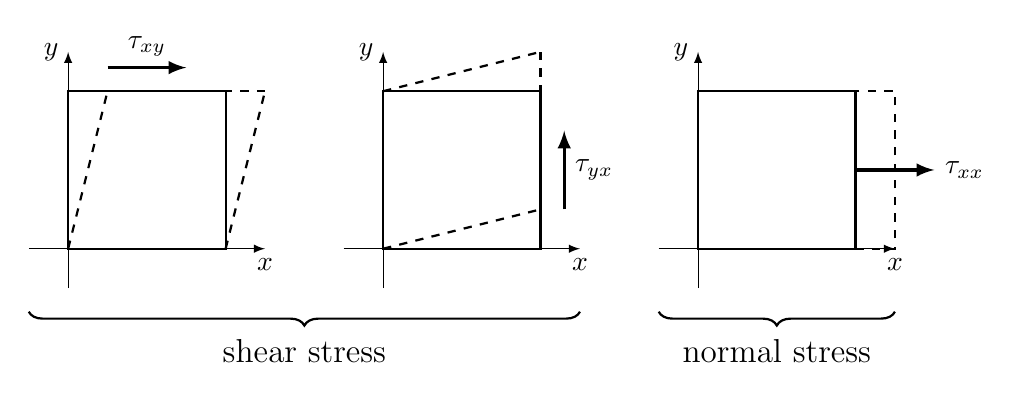
\begin{tikzpicture}[>=latex, scale=1]
        
        % --- STYLE DEFINITIONS ---
        \tikzset{axis/.style={->, thin}}
        \tikzset{solidline/.style={thick}}
        \tikzset{dashedline/.style={thick, dashed}}
        \tikzset{forcearrow/.style={->, very thick}}
        
        % =========================================
        % 1. LEFT DIAGRAM: Shear Stress Tau_xy
        % =========================================
        \begin{scope}[shift={(0,0)}]
            % Axes
            \draw[axis] (-0.5,0) -- (2.5,0) node[below] {$x$};
            \draw[axis] (0,-0.5) -- (0,2.5) node[left] {$y$};
            
            % Original Element (Solid)
            \draw[solidline] (0,0) rectangle (2,2);
            
            % Deformed Element (Dashed) - Shear in x
            % Bottom fixed, top moves right
            \draw[dashedline] (0,0) -- (0.5,2); % Left side
            \draw[dashedline] (2,0) -- (2.5,2); % Right side
            \draw[dashedline] (0.5,2) -- (2.5,2); % Top side (shifted)
            
            % Shear Stress Arrow (on top face)
            \draw[forcearrow] (0.5, 2.3) -- (1.5, 2.3) node[midway, above] {$\tau_{xy}$};
        \end{scope}

        % =========================================
        % 2. MIDDLE DIAGRAM: Shear Stress Tau_yx
        % =========================================
        \begin{scope}[shift={(4,0)}]
            % Axes
            \draw[axis] (-0.5,0) -- (2.5,0) node[below] {$x$};
            \draw[axis] (0,-0.5) -- (0,2.5) node[left] {$y$};
            
            % Original Element (Solid)
            \draw[solidline] (0,0) rectangle (2,2);
            
            % Deformed Element (Dashed) - Shear in y
            % Left fixed, right moves up
            \draw[dashedline] (0,0) -- (2,0.5); % Bottom side
            \draw[dashedline] (0,2) -- (2,2.5); % Top side
            \draw[dashedline] (2,0.5) -- (2,2.5); % Right side (shifted)
            
            % Shear Stress Arrow (on right face)
            \draw[forcearrow] (2.3, 0.5) -- (2.3, 1.5) node[midway, right] {$\tau_{yx}$};
        \end{scope}

        % =========================================
        % 3. RIGHT DIAGRAM: Normal Stress Tau_xx
        % =========================================
        \begin{scope}[shift={(8,0)}]
            % Axes
            \draw[axis] (-0.5,0) -- (2.5,0) node[below] {$x$};
            \draw[axis] (0,-0.5) -- (0,2.5) node[left] {$y$};
            
            % Original Element (Solid)
            \draw[solidline] (0,0) rectangle (2,2);
            
            % Deformed Element (Dashed) - Extension in x
            \draw[dashedline] (2,0) -- (2.5,0) -- (2.5,2) -- (2,2);
            
            % Normal Stress Arrow (on right face)
            \draw[forcearrow] (2, 1.0) -- (3.0, 1.0) node[right] {$\tau_{xx}$};
        \end{scope}

        % =========================================
        % LABELS AND TEXT
        % =========================================
        
        % Braces and Text for Shear Stress (Left & Middle)
        \draw [decorate,decoration={brace,amplitude=5pt,mirror}, thick] (-0.5,-0.8) -- (6.5,-0.8);
        \node at (3, -1.3) {\large shear stress};
        
        % \node[align=left, font=\small] at (3, -2.5) {
        %     \textit{first subscript denotes direction} \\
        %     \textit{shear stress acts; second subscript} \\
        %     \textit{denotes plane normal to line of action}
        % };

        % Braces and Text for Normal Stress (Right)
        \draw [decorate,decoration={brace,amplitude=5pt,mirror}, thick] (7.5,-0.8) -- (10.5,-0.8);
        \node at (9, -1.3) {\large normal stress};
        
        % \node[align=left, font=\small] at (9, -2.2) {
        %      \textit{sometimes denoted by $\sigma_{xx}$ too} 
        % };

    \end{tikzpicture}
